% mnras_template.tex 
%
% LaTeX template for creating an MNRAS paper
%
% v3.0 released 14 May 2015
% (version numbers match those of mnras.cls)
%
% Copyright (C) Royal Astronomical Society 2015
% Authors:
% Keith T. Smith (Royal Astronomical Society)

% Change log
%
% v3.0 May 2015
%    Renamed to match the new package name
%    Version number matches mnras.cls
%    A few minor tweaks to wording
% v1.0 September 2013
%    Beta testing only - never publicly released
%    First version: a simple (ish) template for creating an MNRAS paper

%%%%%%%%%%%%%%%%%%%%%%%%%%%%%%%%%%%%%%%%%%%%%%%%%%
% Basic setup. Most papers should leave these options alone.
\documentclass[fleqn,usenatbib]{mnras}

% MNRAS is set in Times font. If you don't have this installed (most LaTeX
% installations will be fine) or prefer the old Computer Modern fonts, comment
% out the following line
\usepackage{newtxtext,newtxmath}
% Depending on your LaTeX fonts installation, you might get better results with one of these:
%\usepackage{mathptmx}
%\usepackage{txfonts}

% Use vector fonts, so it zooms properly in on-screen viewing software
% Don't change these lines unless you know what you are doing
\usepackage[T1]{fontenc}

% Allow "Thomas van Noord" and "Simon de Laguarde" and alike to be sorted by "N" and "L" etc. in the bibliography.
% Write the name in the bibliography as "\VAN{Noord}{Van}{van} Noord, Thomas"
\DeclareRobustCommand{\VAN}[3]{#2}
\let\VANthebibliography\thebibliography
\def\thebibliography{\DeclareRobustCommand{\VAN}[3]{##3}\VANthebibliography}


%%%%% AUTHORS - PLACE YOUR OWN PACKAGES HERE %%%%%

% Only include extra packages if you really need them. Common packages are:
\usepackage{graphicx}	% Including figure files
\usepackage{amsmath}	% Advanced maths commands
%\usepackage{amssymb}	% Extra maths symbols

%%%%%%%%%%%%%%%%%%%%%%%%%%%%%%%%%%%%%%%%%%%%%%%%%%

%%%%% AUTHORS - PLACE YOUR OWN COMMANDS HERE %%%%%

% Please keep new commands to a minimum, and use \newcommand not \def to avoid
% overwriting existing commands. Example:
%\newcommand{\pcm}{\,cm$^{-2}$}	% per cm-squared

%%%%%%%%%%%%%%%%%%%%%%%%%%%%%%%%%%%%%%%%%%%%%%%%%%

%%%%%%%%%%%%%%%%%%% TITLE PAGE %%%%%%%%%%%%%%%%%%%

% Title of the paper, and the short title which is used in the headers.
% Keep the title short and informative.
\title[Kilonova modeling with SNEC]{Radiation hydrodynamics modeling of kilonovae with SNEC}

% The list of authors, and the short list which is used in the headers.
% If you need two or more lines of authors, add an extra line using \newauthor
\author[Z.~Wu]{
Zhenyu Wu,$^{1}$\thanks{E-mail: 171840687\@smail.nju.edu.cn}
Full author list TBD
\\
% List of institutions
$^{1}$ Nanjing University\\
}

% These dates will be filled out by the publisher
\date{Accepted XXX. Received YYY; in original form ZZZ}

% Enter the current year, for the copyright statements etc.
\pubyear{2021}

% Don't change these lines
\begin{document}
\label{firstpage}
\pagerange{\pageref{firstpage}--\pageref{lastpage}}
\maketitle

% Abstract of the paper
\begin{abstract}
\textcolor{red}{Draft version, not for distribution}
\end{abstract}

% Select between one and six entries from the list of approved keywords.
% Don't make up new ones.
\begin{keywords}
keyword1 -- keyword2 -- keyword3
\end{keywords}

%%%%%%%%%%%%%%%%%%%%%%%%%%%%%%%%%%%%%%%%%%%%%%%%%%%%%%%%%%%%%%%%%%%%%%%%%%%%%

\begin{enumerate}
    \item Use bibtex keys from INSPIRE. I have a script to generate the bibtex automatically from those
    \item The section titles are just suggestions and will be finalized later
    \item Let's start with assembling the relevant plots and some text for the methods section
\end{enumerate}

% ===========================================================================
\section{Introduction}
% ===========================================================================

% ===========================================================================
\section{Methods}
% ===========================================================================

    \subsection{Brief overview of SNEC} 
    SNEC, the SuperNova Explosion Code, is a spherically symmetric (1D) Lagrangian radiation-hydrodynamics code simulating core-collapse supernova explosion. (\cite{morozova2015light}) After reading in the structure and chemical compositions of a progenitor star and the explosion type, the code calculates its explosion and generates bolometric and multicolor light curves. The code mainly uses Paczynski EOS, namely taking into account the ions, electrons and radiation, and solves Saha equations. The code includes radioactive decay of $^{56}$Ni to power supernovae. Rosseland mean opacity is adopted for radiation transfer. 
    
    Unlike core-collapse supernovae, kilonovae are powered by radioactive decay of heavy elements synthesis through r-process. Modeling the opacities of r-process elements and the heating rates due to their decay is the key to kilonova simulations. Given the complexity of elements in kilonovae, we use the average properties of different compositions, like the initial electron fraction $Y_e$. Moreover, the intial profiles of supernova progenitors in SNEC are from MESA, while we use two kinds of profiles here. We use wind profiles for code validation and comparison with other analytical models. We also have more realistic initial profiles derived from numerical relativity. In the following we will explain the opacities, heating rates, initial and boundary conditions in our code and other differences from SNEC.
    

    \subsection{Opacities} 
     Tanaka et al has done detailed research on opacities of mixture of r-process elements. In (\cite{tanaka2018properties}),  they show that bolometric lightcurves with grey opacity of $1.0$ cm$^2$ g$^{-1}$ and $10.0$ cm$^2$ g$^{-1}$ agree with results using wavelength-dependent radiative transfer. The grey opacity values were also adopted for red, purple and blue kilonova components in (\cite{villar2017combined}) to fit AT2017gfo. In our model, we use grey opacity and set its lower and upper bound to $1.0$ cm$^2$ g$^{-1}$ and $10.0$ cm$^2$ g$^{-1}$ respectively. We set the opacity corresponding to $Y_e \ 0.25$ to the intermediate $5.5$ cm$^2$ g$^{-1}$, and then use a simple smooth function to describe the change of opacity $\kappa$ with $Y_e$:
        
    
    \begin{equation}
    	\label{opacity_ye}
    	\kappa = 1 + \frac{9}{1+(4Y_e)^{12}}~~ \mathrm{ [cm^2 g^{-1}]}
    \end{equation}
    
    Figure \ref{opacity_Ye} shows the comparison of our model with (\cite{tanaka2020systematic}) results. It is worth noting that, for simplicity, the opacity in our model is a constant, namely it doesn't change with time or temperature. In addition, grey opacity's application to multicolor light curves needs further study.
   
    
    \begin{figure}
    \centering
    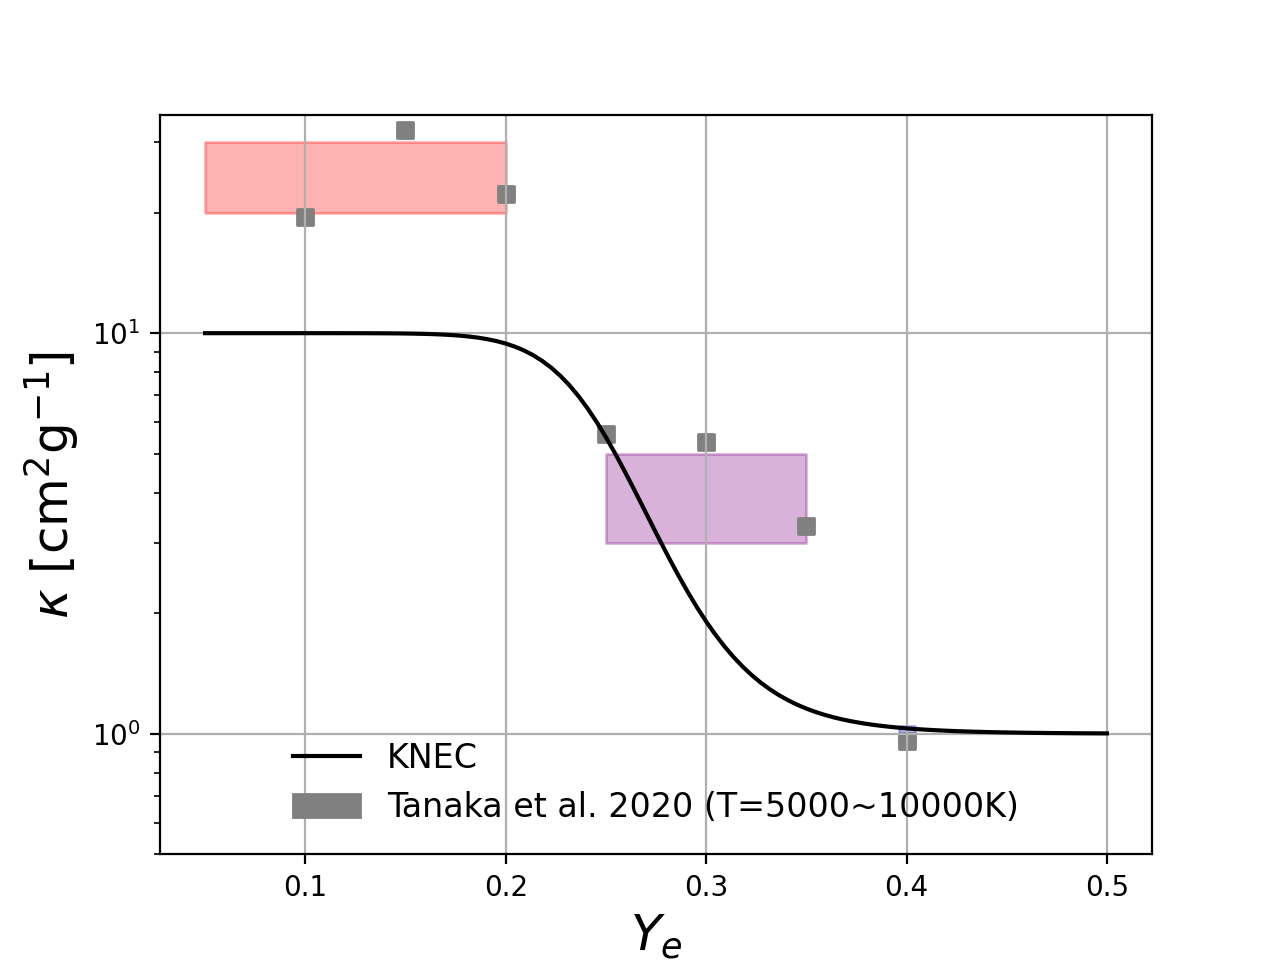
\includegraphics[scale=0.5]{figures/opacity_Ye.png}
    \caption{The solid line is opacity as a function of $Y_e$ in our model  (Equation \ref{opacity_Ye}). Little grey squares show Tanaka et al's data, and the large rectangles are the suggested opacity range in their paper. (at 5000 $\sim$ 10000K, and they decrease steeply at lower temperature.) Opacity in our model is a little lower than their results due to the upper bound $10$ cm$^2$ g$^{-1}$ we set.}
    \label{opacity_Ye}
    \end{figure} 
    


    
    
    
    \subsection{Heating rates}
    At the times relevant for kilonovae, the ejecta has already lost all of its initial thermal energy at expansion, and the dominant source of heating is constituted by the decays of heavy elements produced in the r-process. This heating can be described by a specific heating rate which can be derived by evolving the system of the numerous characteristic nuclides in time while accounting for their mutual interactions.\\
    Here, time-dependent heating rates obtained using the nuclear reaction network SkyNet with a FRDM nuclear mass model are employed. A single SkyNet run is determined by the set of thermodynamic variables initial electron fraction $Y_e$, initial specific entropy $s$ and expansion timescale $\tau$. The rates are thus computed on a comprehensive grid with $0.02\leq Y_e\leq0.48$ linearly spaced, $1.82$ $\mathrm{k_B/baryon}$ $\leq s\leq100$ $\mathrm{k_B/baryon}$ and $1.36$ ms $\leq\tau\leq100$ ms log-spaced, the results on a representative subgrid being reported in Figure \ref{heatrates}.\\
    \begin{figure}
    \centering
    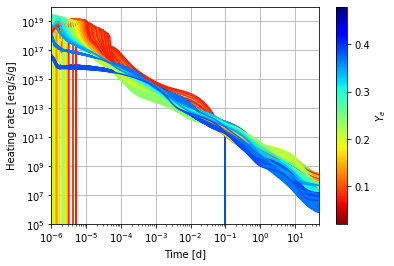
\includegraphics[scale=0.6]{figures/heating/heating rate fits/heatrates.png}
    \caption{Heating rate trajectories as obtained by SkyNet on a subgrid of thermodynamic variables $0.05\leq Y_e\leq0.4$, $3$ $\mathrm{k_B/baryon}$ $\leq s\leq50$ $\mathrm{k_B/baryon}$ and $1$ ms $\leq\tau\leq30$ ms for visual clarity. Trajectories are color-coded to indicate different initial electron fractions. Vertical lines correspond to SkyNet noise which is averaged out in the fit procedure.}
    \label{heatrates}
    \end{figure}
    In order to derive the heating rate for arbitrary initial conditions, the above trajectories are reduced to a parametrized functional form by means of a fit procedure intended to cover the time interval from $0.1$ s to $50$ days post-merger, and, in particular, a distinction between time regimes is introduced. For early times $t\lesssim0.1$ days, the analytic fitting formula, derived from detailed nucleosynthesis calculations (\cite{Korobkin:2012uy}), is employed:
    \begin{equation}
    \label{eqKorfit}
    \dot{\epsilon}_{\mathrm{r}}(t)=\epsilon_0\epsilon_{\mathrm{th}}\left(\frac{1}{2}-\frac{1}{\pi}\arctan{\left[\frac{t-t_0}{\sigma}\right]}\right)^{\alpha},
    \end{equation}
    where $\epsilon_0$, $\alpha$, $t_0$ and $\sigma$ are considered fit parameters, while $\epsilon_{\mathrm{th}}<1$ is the thermalization efficiency. At late times $t\gtrsim0.1$ days instead, we expect a power-law fit to be a sufficiently good approximation of the heating rates, and thus the fitting formula becomes:
    \begin{equation}
    \label{eqpowfit}
    \dot{\epsilon}_{\mathrm{r}}(t)=\epsilon_0'\epsilon_{\mathrm{th}}t^{-\alpha'},
    \end{equation}
    with $\epsilon_0'$ and $\alpha'$ additional fit parameters. The heating rate fits, as obtained by using equations \ref{eqKorfit} and \ref{eqpowfit}, are then joint together with a log-scaled smoothing procedure applied on the time interval $1\times10^3$ s $\leq t\leq4\times10^4$ s, centered on $t\sim0.1$ days in log-scale.\\
    Figure \ref{heatratesfit} shows the fitted version of the heating rate trajectories presented in Figure \ref{heatrates}.
    \begin{figure}
    \centering
    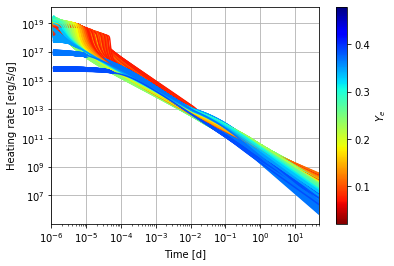
\includegraphics[scale=0.65]{figures/heating/heating rate fits/heatratesfit.png}
    \caption{Heating rate fitted trajectories as obtained by performing the fit procedure on a subgrid of thermodynamic variables $0.05\leq Y_e\leq0.4$, $3$ $\mathrm{k_B/baryon}$ $\leq s\leq50$ $\mathrm{k_B/baryon}$ and $1$ ms $\leq\tau\leq30$ ms for visual clarity. Trajectories are color-coded to indicate different initial electron fractions.}
    \label{heatratesfit}
    \end{figure}
    The quality of a single fit is evaluated using a mean fractional log error, defined as:
    \begin{equation}
    \label{eqlogerror}
    \Delta(\dot{\epsilon}_{\mathrm{r}})=\left<\frac{|\ln(\dot{\epsilon}_{\mathrm{r}}^o(t))-\ln(\dot{\epsilon}_{\mathrm{r}}(t))|}{\ln(\dot{\epsilon}_{\mathrm{r}}^o(t))}\right>,
    \end{equation}
    where $\dot{\epsilon}_{\mathrm{r}}^o(t)$ is the original SkyNet heating rate trajectory, and the mean is performed over the entire time window $0.1$ s $\leq t\leq50$ days. As visible in Figure \ref{fiterror}, our fit procedure returns considerably accurate results: the vast majority of trajectories are reproduced within $\sim1\%$ relative error, while the worst cases, corresponding to external points in the input grid, carry only a slightly higher error $\lesssim 5\%$.
    \begin{figure}
    \centering
    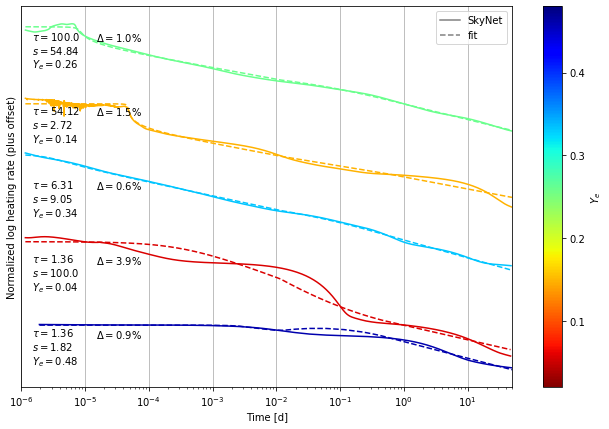
\includegraphics[scale=0.4]{figures/heating/heating rate fits/fiterror.png}
    \caption{Heating rate SkyNet trajectory along with its fitted version for five different representative sets of thermodynamic variables. Each fit is matched with its relative error defined by equation \ref{eqlogerror}. Trajectories are color-coded to indicate different initial electron fractions.}
    \label{fiterror}
    \end{figure}
    
    
    \subsection{Initial and boundary conditions} 
    
   \subsubsection{Initial ejecta profiles}
    The initial profiles contain the following information about the ejecta: {\it mass, radius, temperature, density, velocity, $Y_e$, entropy, }and {\it expansion timescale}. Compared to profiles for the original SNEC code, entropy and expansion timescale are our new additions in order to calculate heating rates more accurately. All these ejecta properties can be obtained from numerical relativistic simulations of binary neutron star mergers. For example, the SFHo profile and BLh profile are derived from equatorial ejecta about 0.1 s after NS-NS merger. See Figure \ref{blh_profile} for the properties of BLh profile. 
    
    Besides the realistic SFHo and BLh profiles, we design simple wind profiles for numerical experiments and comparison with analytical models. We use a model similar to those introduced in \cite{metzger2010electromagnetic} and \cite{tanaka2013radiative}. Velocity $v \propto r$ and ranges between 0.05 c and 0.2 c, while density $\rho \propto r^{-3}$. The maximum radius is set to $10^{9}$ cm and the total mass is 0.01 solar mass by default. We call it {\it wind3} profile, indicating the powerlaw index 3 in density. Initial temperature $T$, electron fraction $Y_e$, entropy $s$ and expansion timescale $\tau$ are uniform in the ejecta, with $T$ set to $10^9$ K by default. 
    
    Furthermore, we improve the wind3 profile with another powerlaw index for density near the outer boundary, which is the method used in \cite{ishizaki2021fallback}. We set the second powerlaw index to 8 to model the sharp decrease in density near the outer boundary. We call it wind38 profile,  see Figure \ref{wind3_wind38_profile} for details.
   
    
    
    \begin{figure}
    \centering
    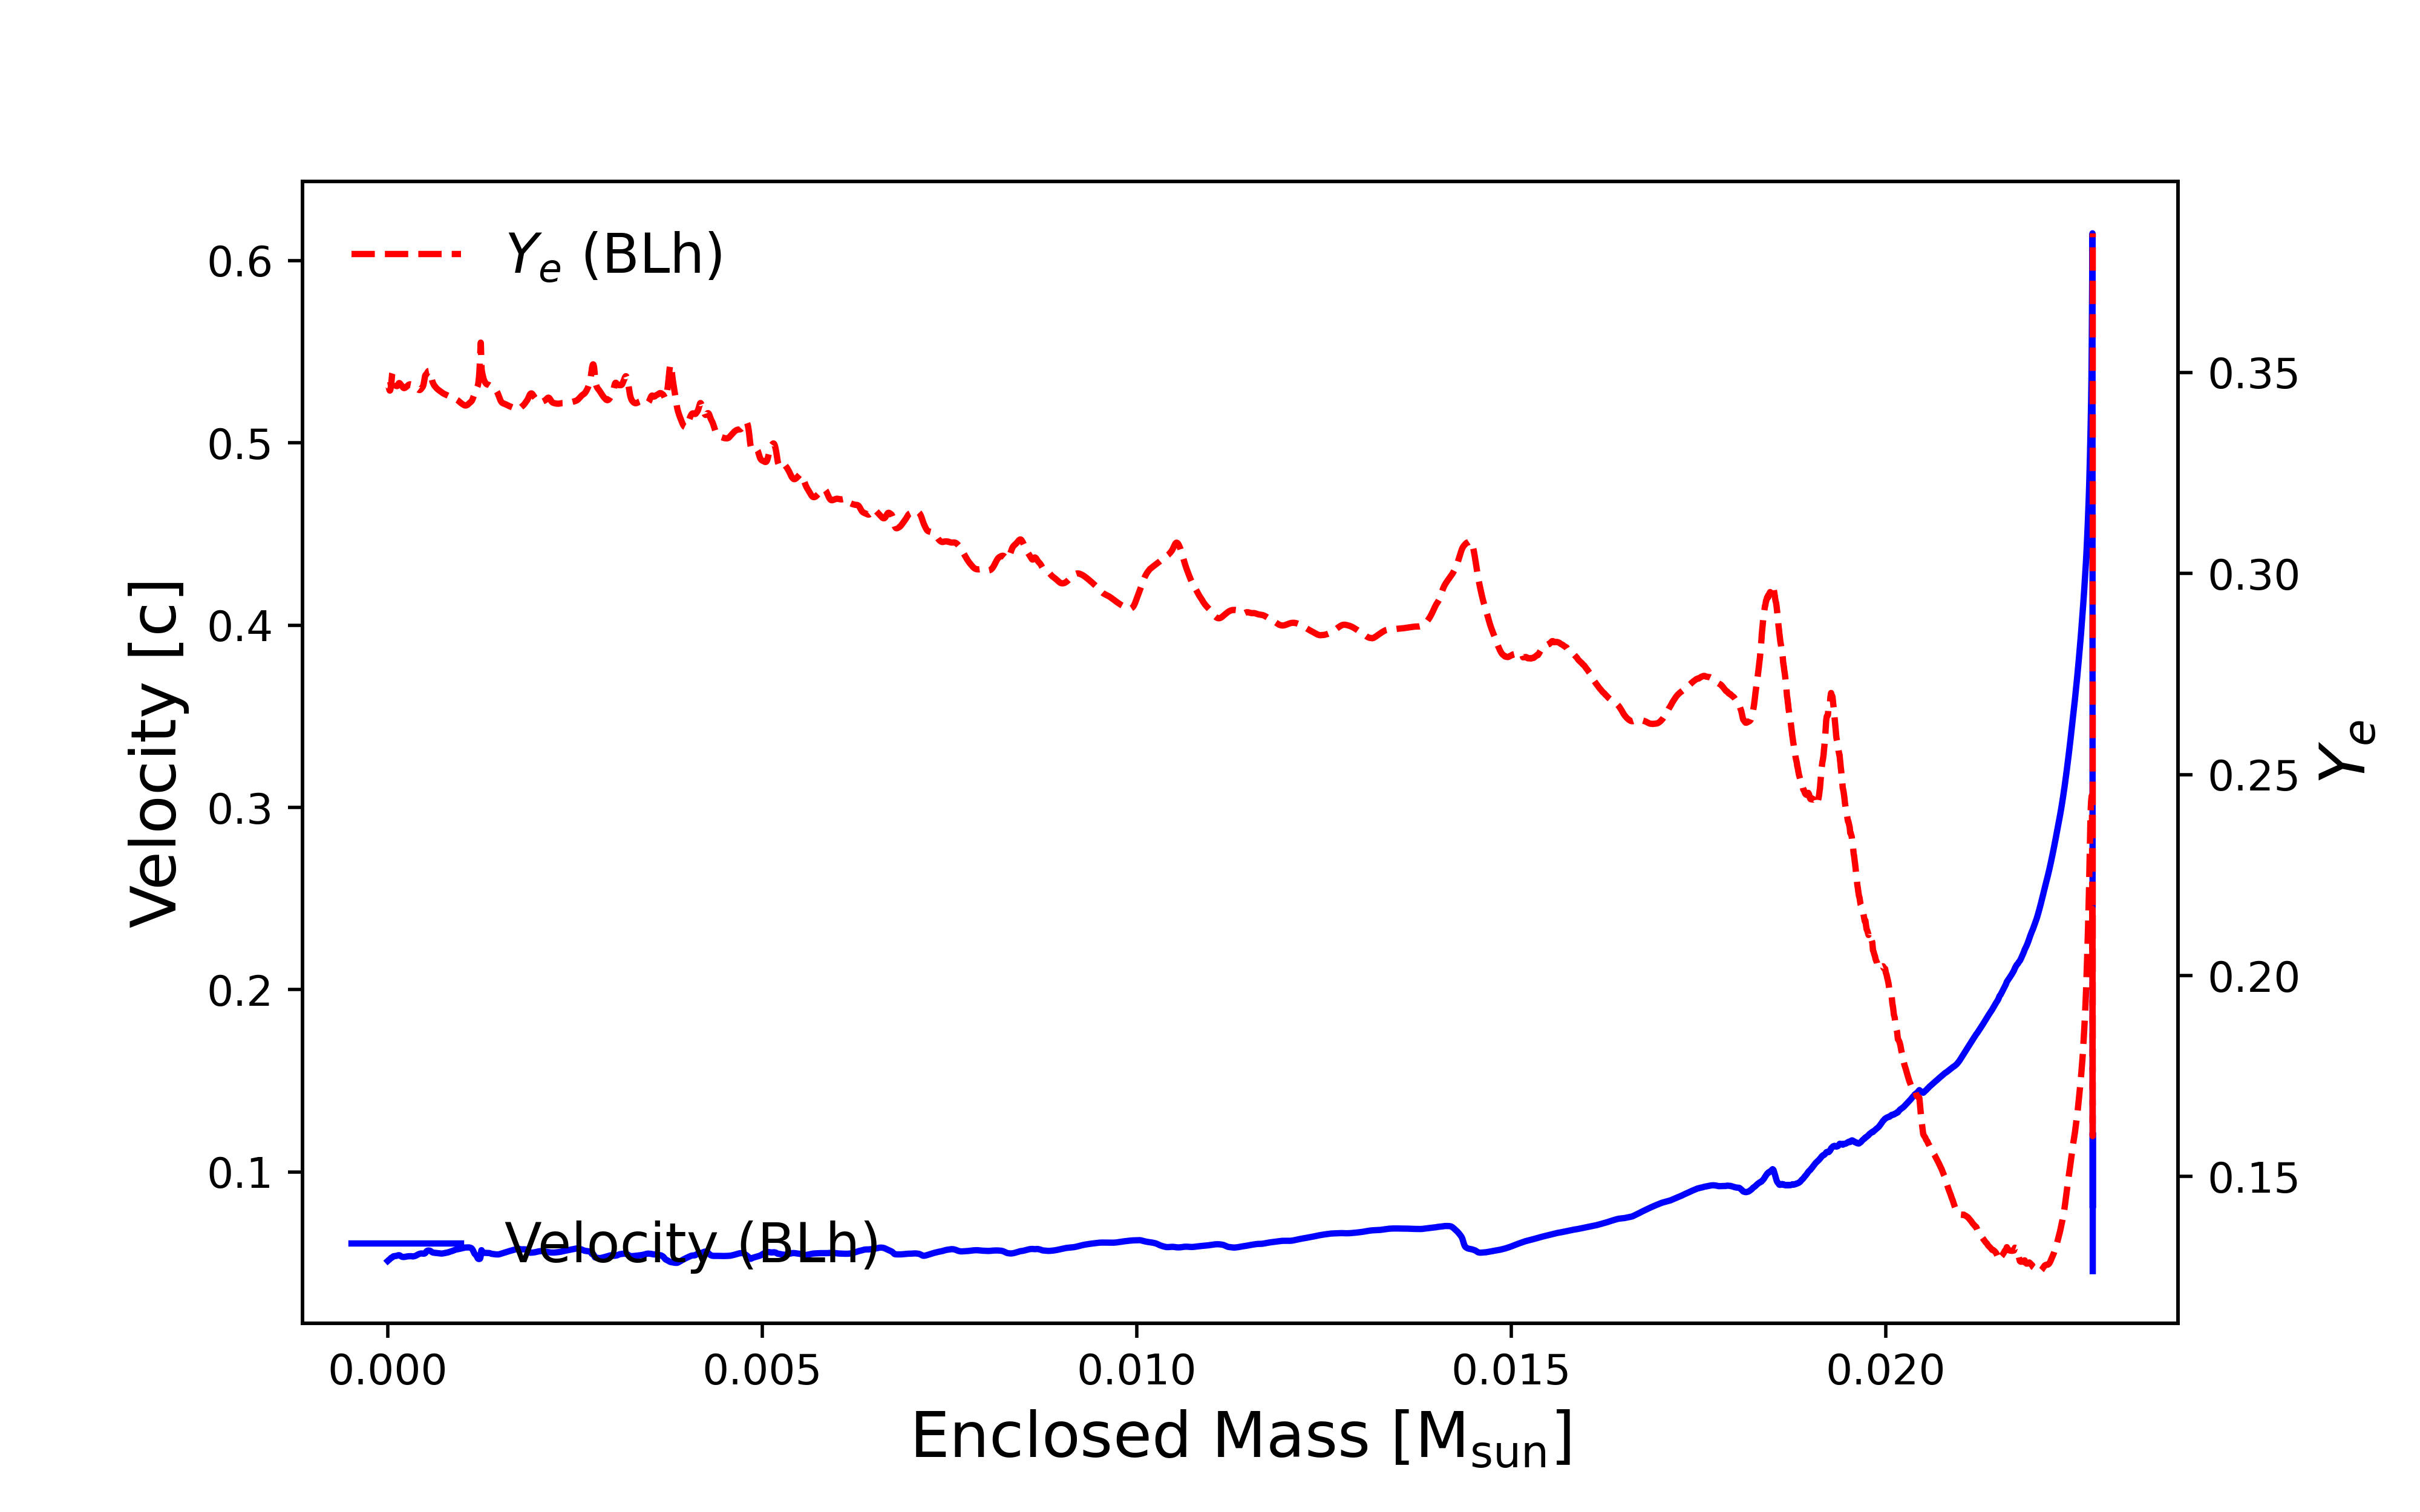
\includegraphics[scale=0.4]{figures/profiles/blh_vel_ye_mass.png}
    \caption{BLh profile: velocity and $Y_e$ as a function of mass. (0.12 s after merger, when the innermost of the ejecta passes r = 295 km.) Velocity almost keeps constant but rises sharply to $\sim$ 0.6 c at the outer boundary. In general, the inner part has higher $Y_e$, but there is a high-$Y_e$ front at the outer boundary.}
    \label{blh_profile}
    \end{figure}
    
        
    \begin{figure}
    \centering
    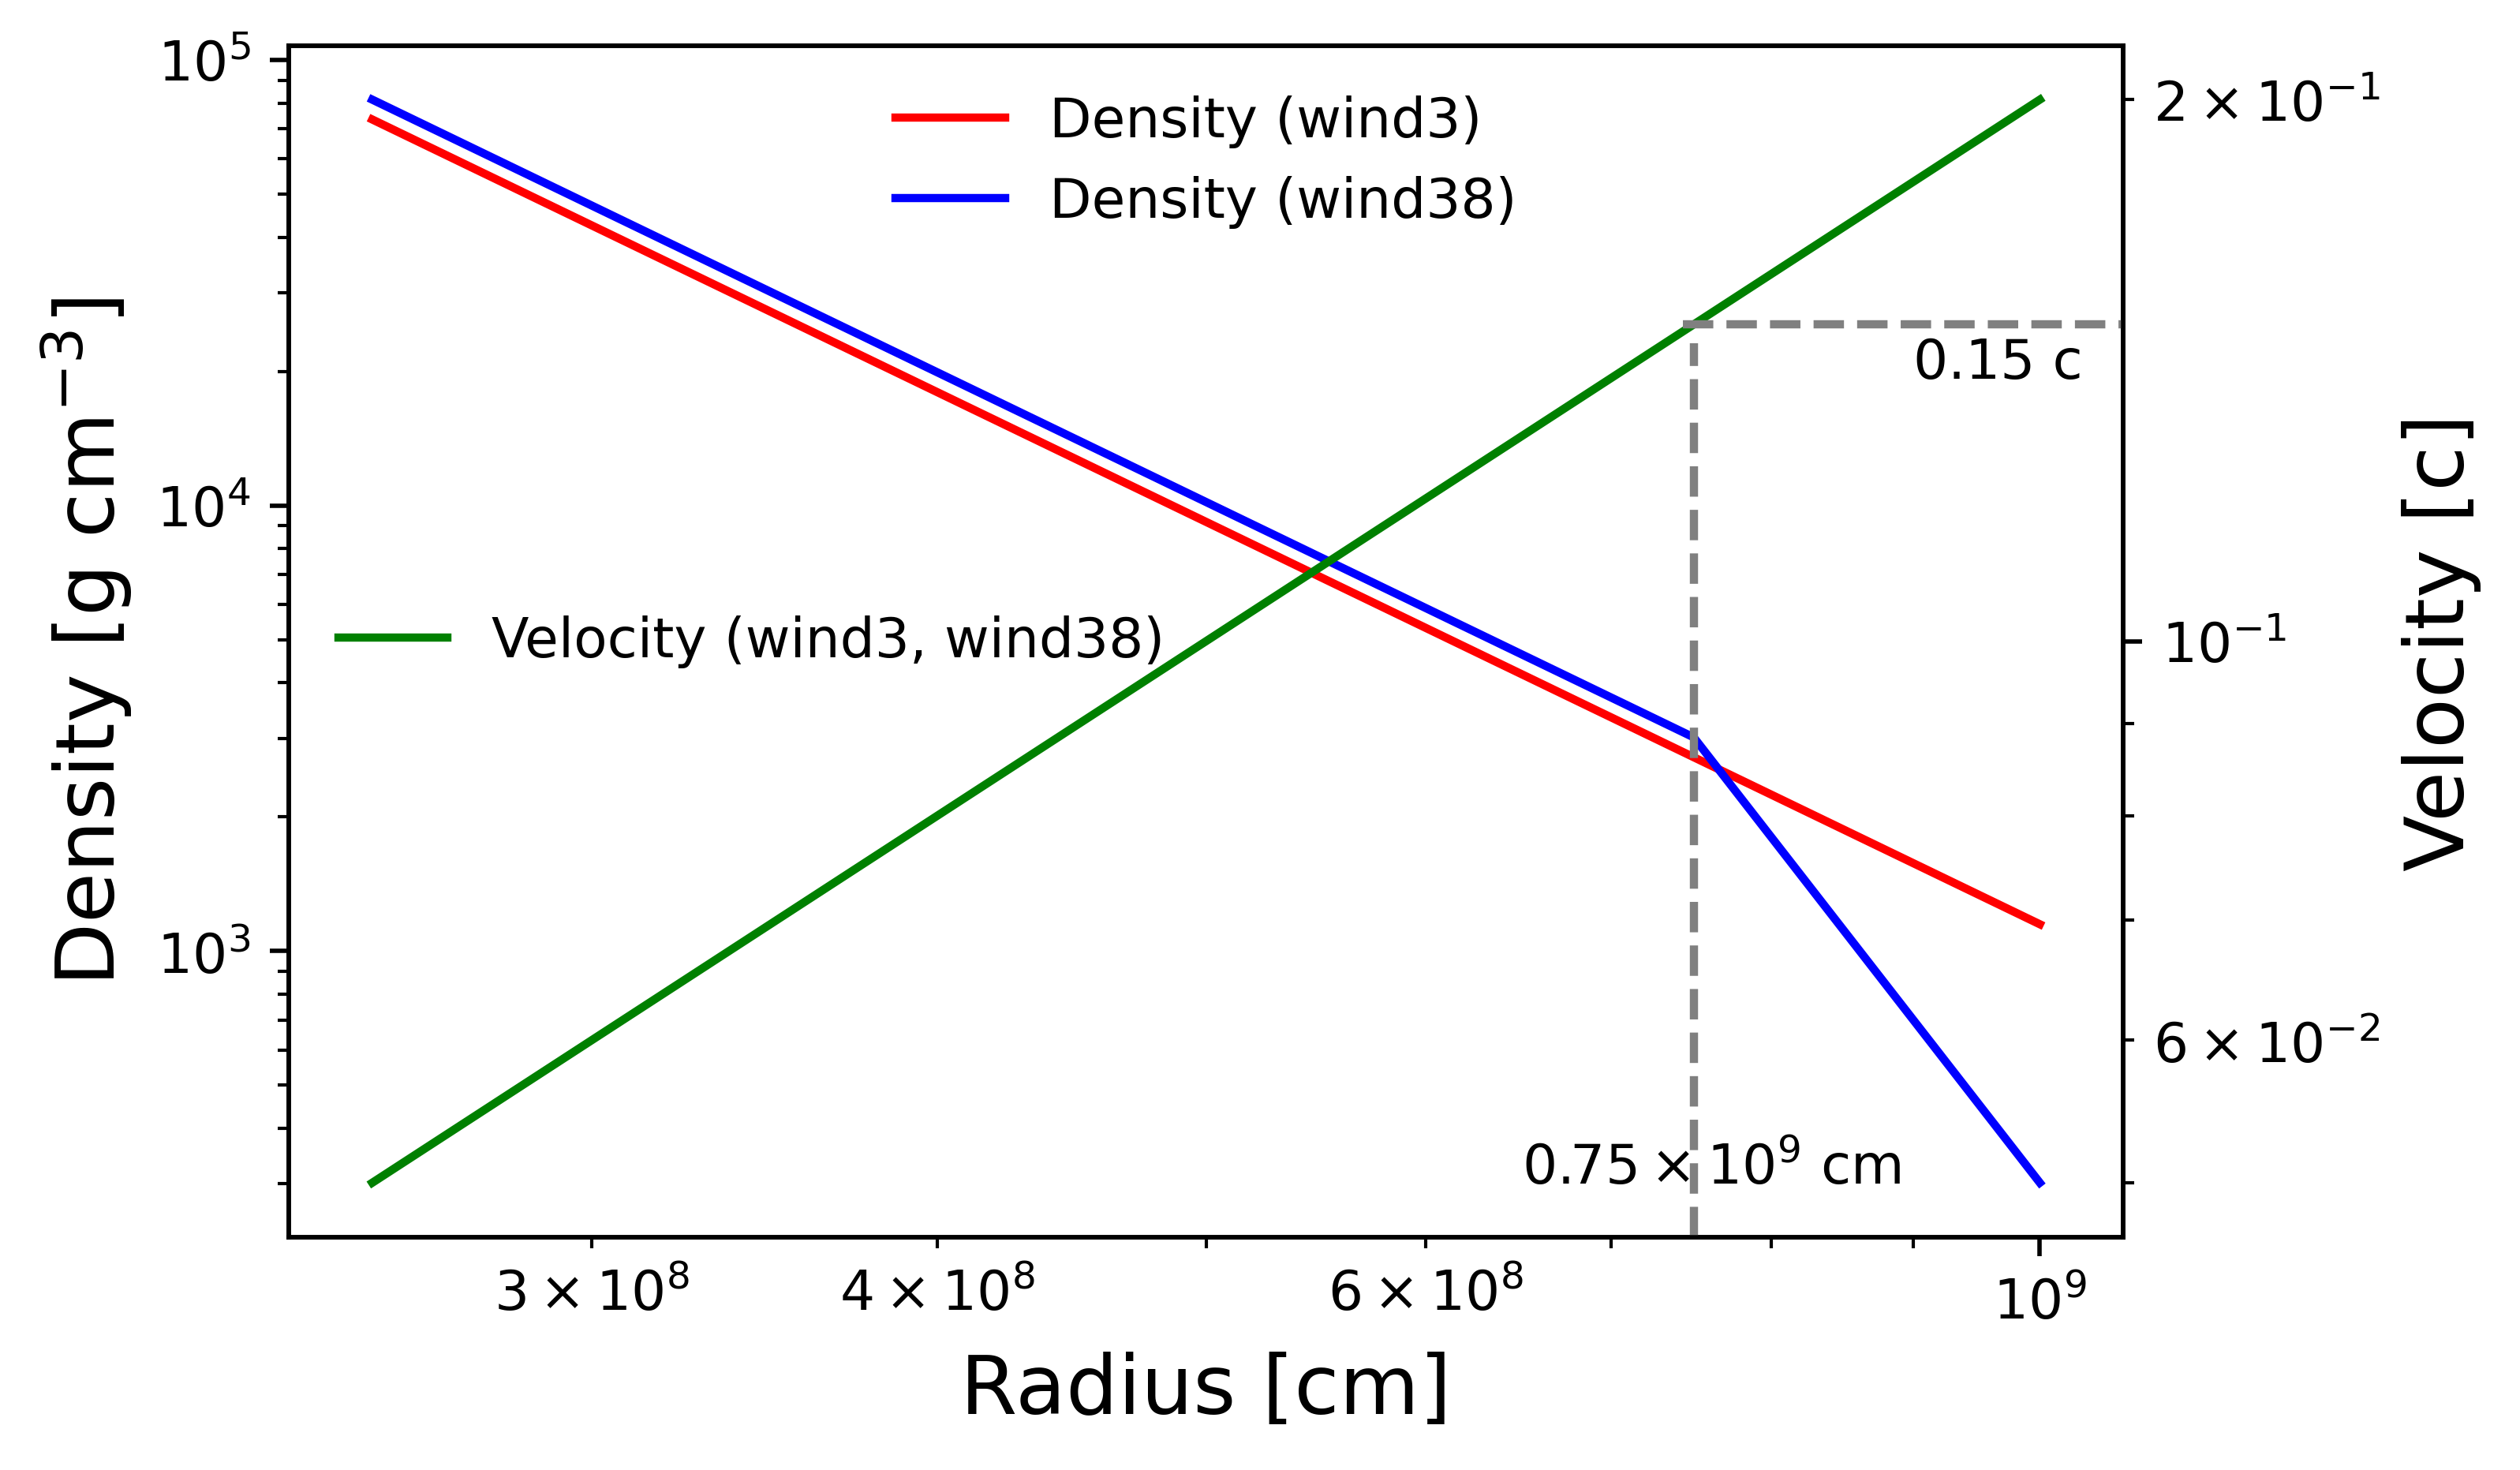
\includegraphics[scale=0.5]{figures/profiles/wind3_wind38_profile.png}
    \caption{wind3/wind38 profile: density and velocity. For wind38 profile, $v \propto r$, $\rho \propto r^{-3}$ when $v \le 0.15$ c, $\rho \propto r^{-8}$ when $v \ge 0.15$ c. The total mass for both wind3 and wind38 profile is 0.01 solar mass.}
    \label{wind3_wind38_profile}
    \end{figure}
    
    
   \subsubsection{Boundary conditions}
 
   At the inner boundary (i = 1), we keep the velocity constant: $v_1 = v_1(t=0)$. Other boundary conditions are the same as SNEC default. At the outer boundary (i = imax), the only active boundary condition, i.e., the boundary condition affecting SNEC hydrodynamical evolution, is pressure $p_{imax}$, while other quantities like temperature $T_{imax}$ and specific internal energy $\epsilon_{imax}$ are passive. We use $p_{imax} = 0$ boundary condition. But this can lead to velocity near outer boundary diverging. (See Figure \ref{boundary_velocity}). One way to solve this divergency problem is to use $p_{imax}$ = $p_{imax-1}$ boundary condition instead, but this causes pdV term at boundary accounting for $\sim$ 20\% in energy conservation, which is what we don't want. Therefore, we continue to use $p_{imax}$ = 0 boundary condition, and we will examine its influences to light curves later.    
   
    \begin{figure}
    \centering
    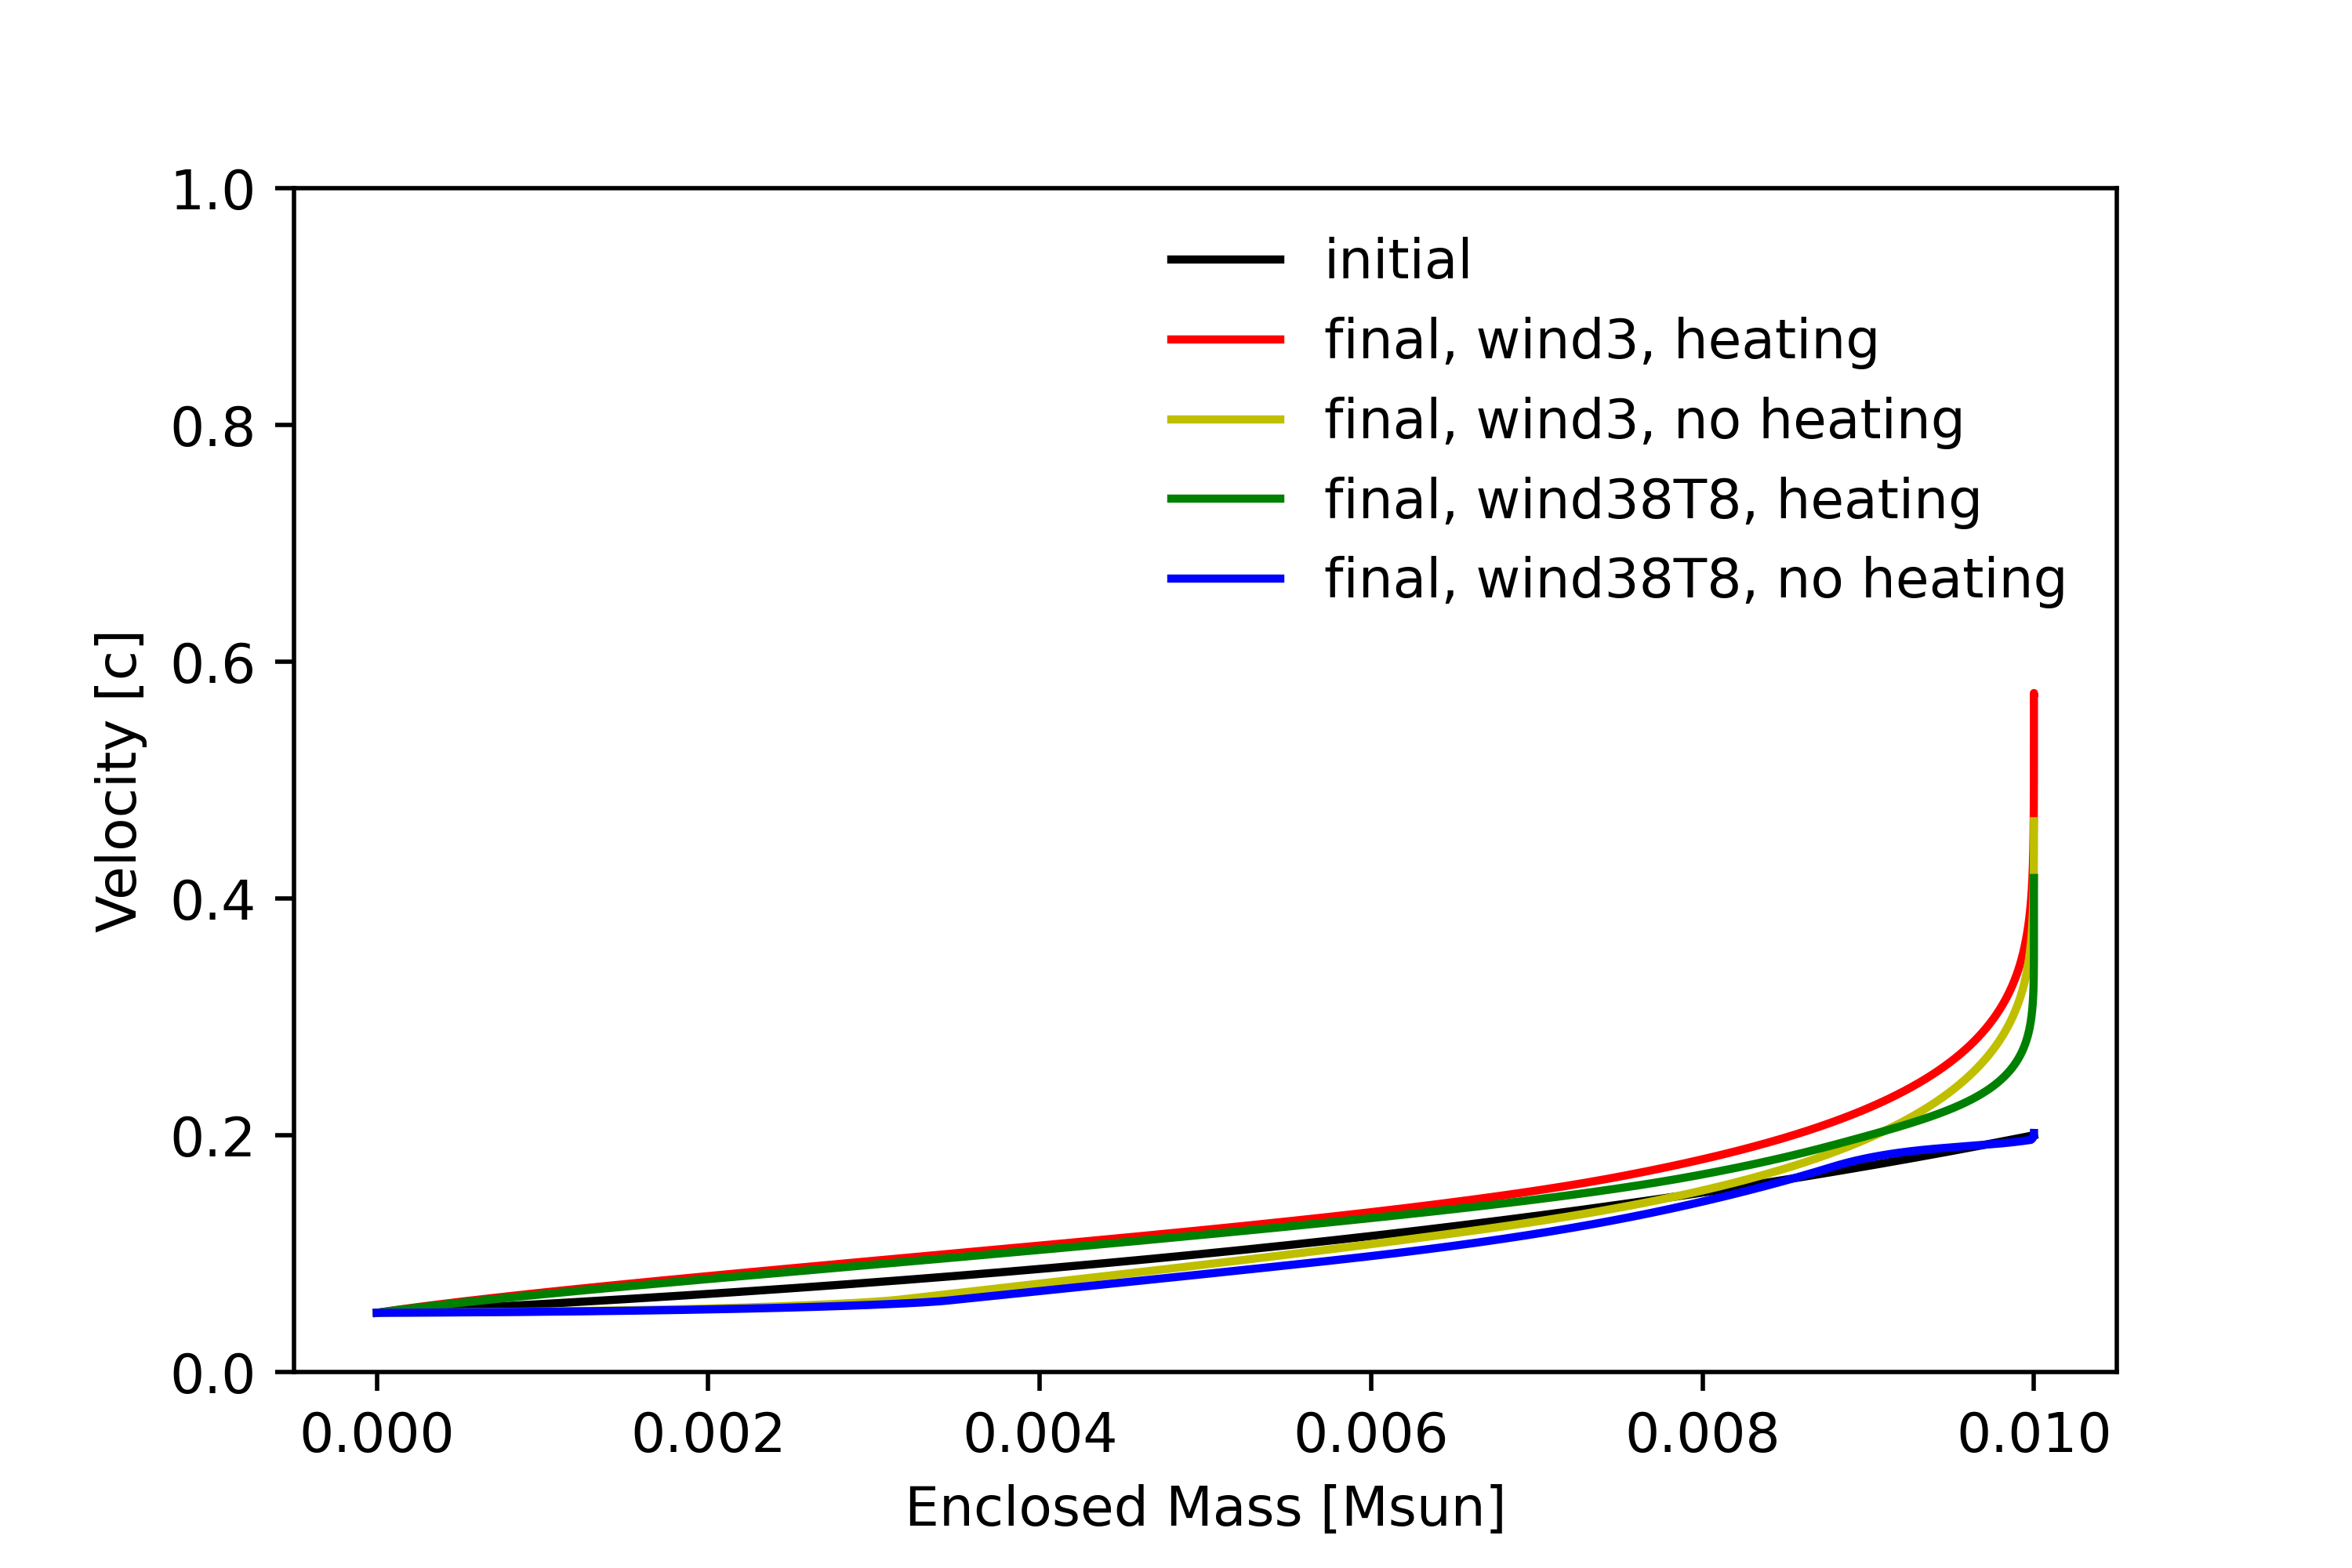
\includegraphics[scale=0.5]{figures/boundary/outer_boundary_velocity}
    \caption{check boundary effects to velocity}
    \label{boundary_velocity}
    \end{figure}    

    \begin{figure}
    \centering
    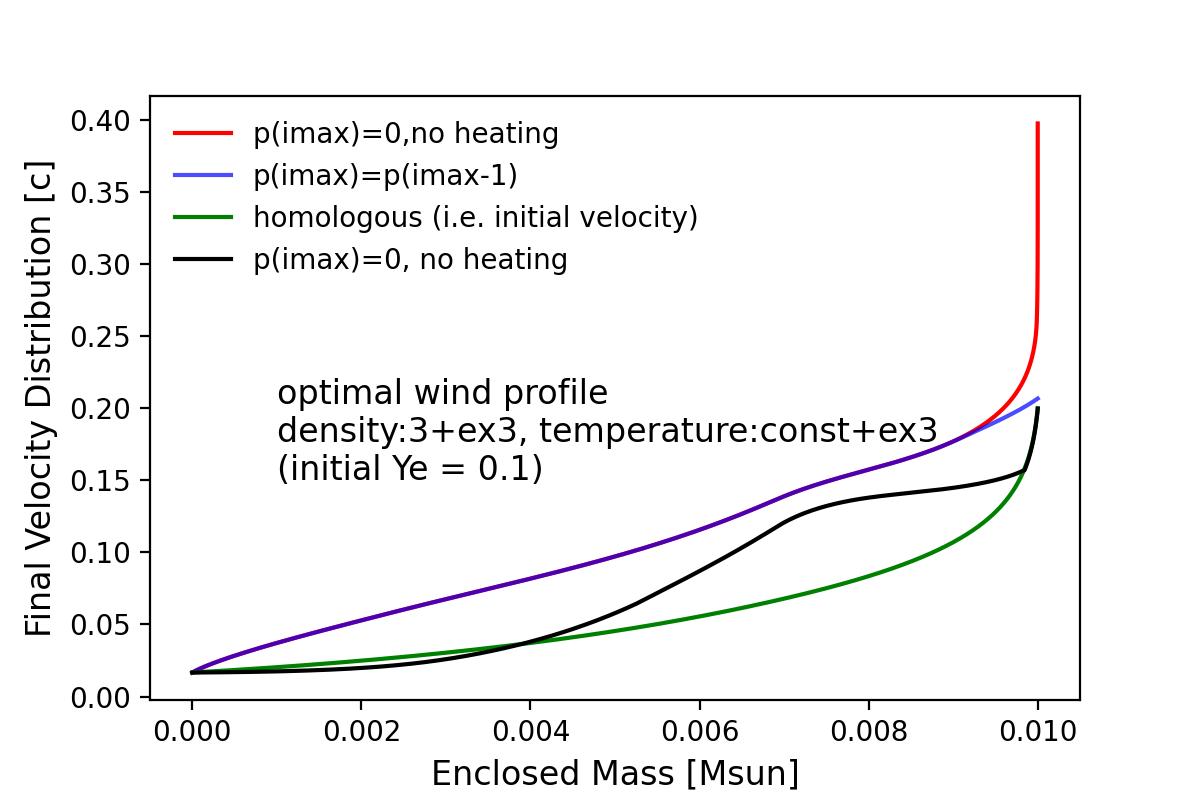
\includegraphics[scale=0.5]{figures/boundary/boundary_velocity_wind3ex3-Tex3.png}
    \caption{boundary velocity: optimal wind}
    \label{boundary_velocity_optimal_wind}
    \end{figure}   
    
    
    \begin{figure}
    \centering
    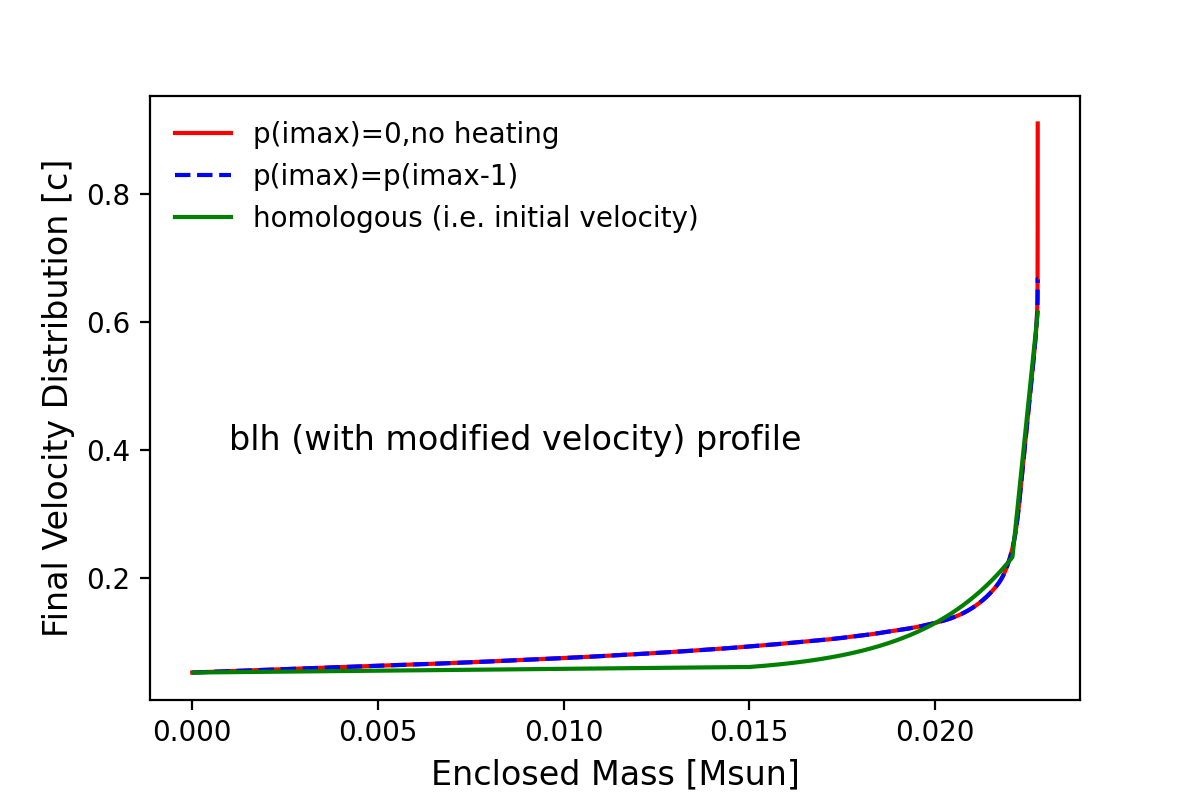
\includegraphics[scale=0.5]{figures/boundary/boundary_velocity_blh-mvel.png}
    \caption{boundary velocity: blh (with modified velocity)}
    \label{boundary_velocity_blh-mvel}
    \end{figure} 




    \subsection{Other differences from SNEC}
    
    \begin{itemize}
        \item Composition and EOS \\
        Due to the complexity of elements in the ejecta, we no longer use the composition profile, but use their average properties like $Y_e$ and entropy instead. We use a simplified Paczynski EOS, ignoring thehttps://www.overleaf.com/project/604ebc5546f3cbe68dd006f9 correction terms for ionization. Saha equations are not solved. The mean degree of ionization $\bar y$ is a free parameter in our model. Another additional free parameter in EOS is the mean molecular weight $\mu$. The default value of $\bar y$ and $\mu$ in our model is 2 and 100 respectively. We find they have little impact on light curves. (see Figure and Figure)
        
        \begin{figure}
        \centering
        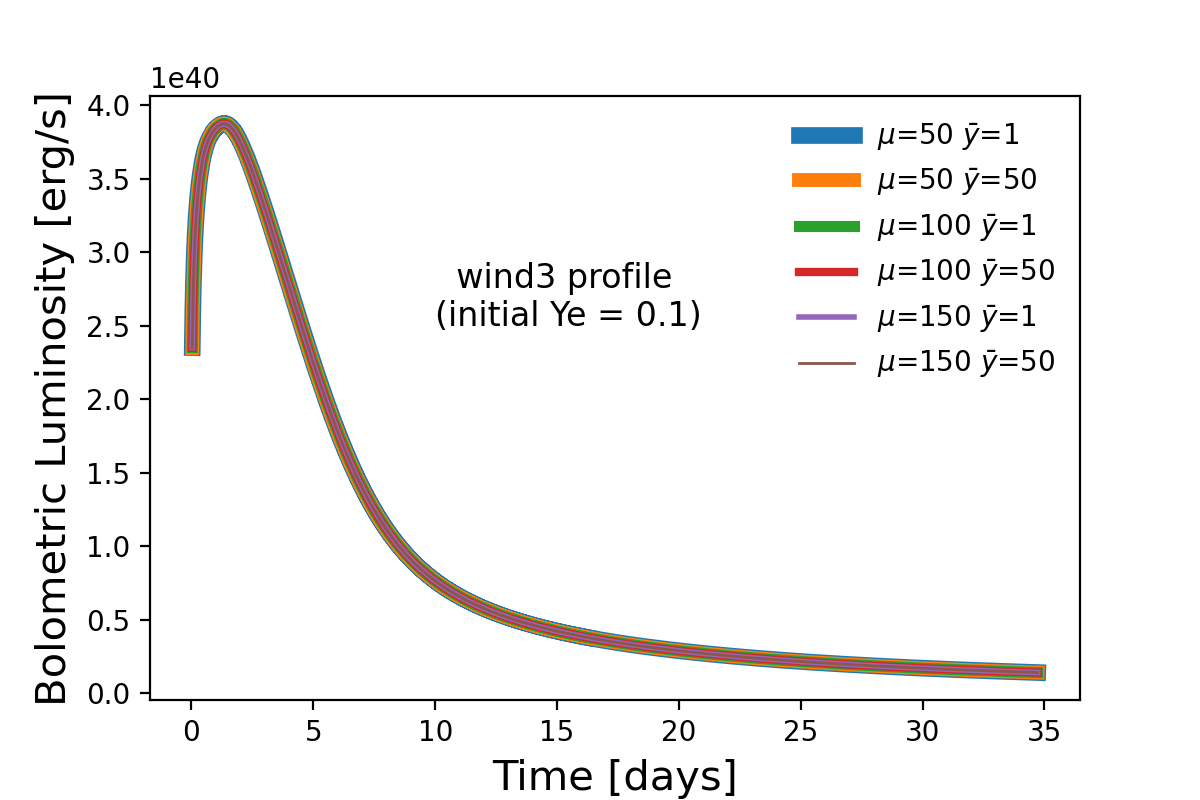
\includegraphics[scale=0.5]{figures/EOSimpact/Effects_mu_ybar_wind3.png}
        \caption{Effects of mean molecular weight and average degree of ionization. Using wind3 profile, we traverse the parameter space of mean molecular weight $\mu$ and average degree of ionization $\bar{y}$, with $\mu$ in [50, 100, 150] and $\bar{y}$ in [1, 2, 10, 50] respectively. We find that they have little impacts on bolometric light curves. }
        \label{Effects_mu_ybar_wind3}
        \end{figure} 
       
          
      
    	\item Explosion setup \\
    	SNEC provides two Explosion types: Thermal Bomb and Piston Explosion. However, since our initial ejecta profiles are derived from numerical simulations or designed wind profiles, there is no need to set up explosions additionally. So we simply set the explosion type to Thermal Bomb and set the energy input to 0. Also, we don't need the boxcar in SNEC to mimic element mixing due to explosion.
    	
    
    	\item Central Remnant \\
    	The central remnant after merger provides external gravitational pull to the ejecta. Its mass is 3 solar mass, typical for NS-NS merger, in our model.
    	
    \end{itemize}
    

    \subsection{Bolometric luminosities and Multicolor luminosities} 
    
    Blackbody radiation assumption for kilonovae is commonly used in previous research, such as the single-temperature model in (\cite{li1998transient}), and multi-component model in (\cite{villar2017combined}). Non-thermal radiation is negligible at $T \sim$ 5000 $K$, although it may become important at late times when the ejecta becomes transparent (\cite{kasen2013opacities},  \cite{tanaka2013radiative}). 
    
    To model bolometric and multi-band light curves, we use a multi-temperature blackbody model here, assuming that the photosphere and each shell above it emit blackbody radiation. Similar to the original SNEC code, bolometric luminosity is expressed as:
    \begin{equation}
        L_{\mathrm{bol}} =  L_{\mathrm{ph}} + \sum_{i=i_{\mathrm{ph}}}^{imax} \dot{\epsilon_i} \Delta m_i 
    \label{Lbol} 
    \end{equation}
    where $L_{\mathrm{ph}}$ is the luminosity at photosphere and $i_{\mathrm{ph}}$ is the cell index of photosphere. $\dot{\epsilon_i}$ is the heating rate including thermalization efficiency in the ith cell.  
    
    The observed flux density at frequency $\nu$ is
    \begin{equation}
       	f_{\nu,obs} = \frac{L_{\mathrm{ph}}}{4 \pi D^2} \frac{\frac{2h \nu^3}{c^2} \frac{1}{e^{h \nu /k_{\mathrm{B}} T_{\mathrm{ph}}}-1}}{\sigma T_{\mathrm{ph}}^4 / \pi}  + \sum_i \frac{\dot{ \epsilon_i} \Delta m_i}{4 \pi D^2} \frac{\frac{2h \nu^3}{c^2} \frac{1}{e^{h \nu /k_{\mathrm{B}} T_i}-1}}{\sigma T_i^4 / \pi} 
    \end{equation}
    where $\sigma$ is the Stefan–Boltzmann constant, and we set the distance $D$ between the kilonova event and the observer to 40 Mpc. We use AB magnitude system in our simulations:   
	\begin{equation}
    m_{\mathrm{AB}} \approx-2.5 \log _{10}\left(\frac{\int f_{\nu}(h \nu)^{-1} e(\nu) \mathrm{d} \nu}{\int 3631 \mathrm{Jy}(h \nu)^{-1} e(\nu) \mathrm{d} \nu}\right)
	\end{equation}
    The filters $e(\nu)$ are downloaded from the SVO Filter Profile Service\footnote{\label{foot:filters}\url{http://svo2.cab.inta-csic.es/theory/fps/}}, and we mainly use CTIO and Gemini bands.
% ===========================================================================
\section{Code validation}



% ===========================================================================
\subsection{Hydrodynamics}

\begin{figure}
\centering
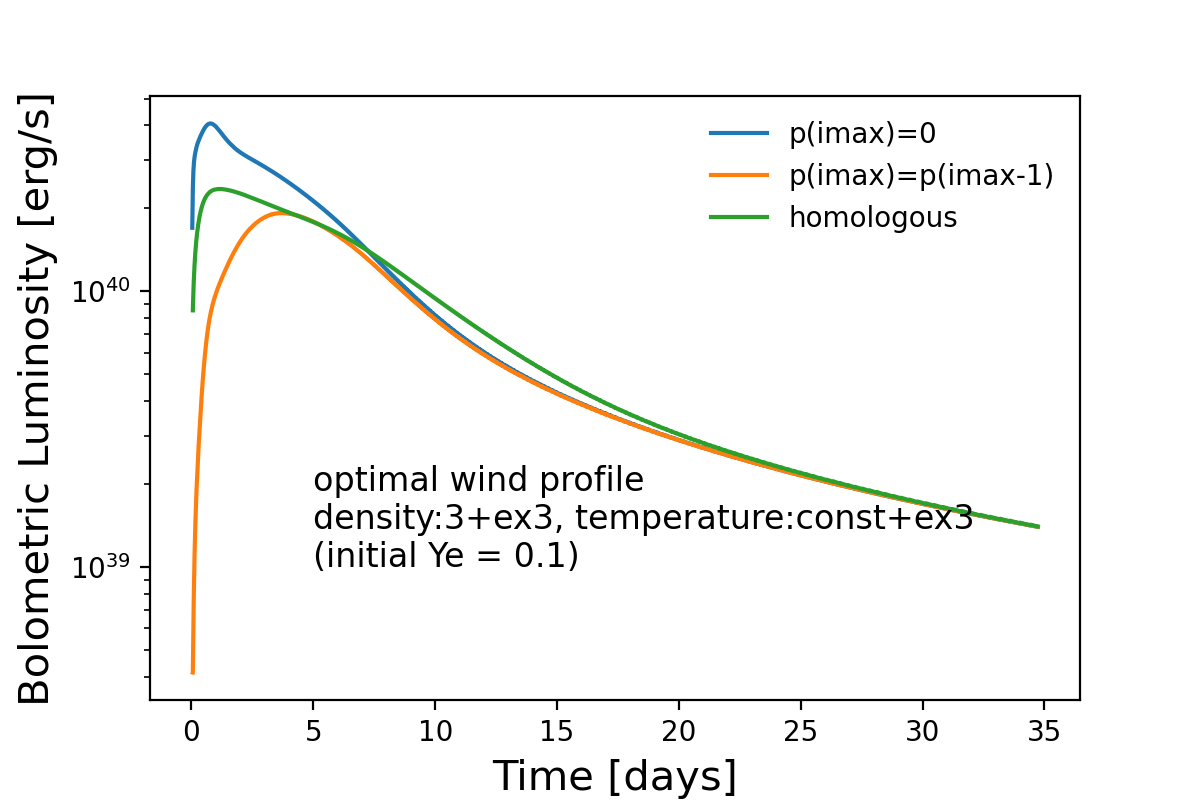
\includegraphics[scale=0.5]{figures/CodeValidation-Hydrodynamics/LC_wind3ex3-Tex3_cb_zb_homologous.png}
\caption{Homologous Expansion VS Hydrodynamic Evolution: optimal wind profile}
\label{CodeValidation-Hydro_wind3ex3-Tex3}
\end{figure} 

\begin{figure}
\centering
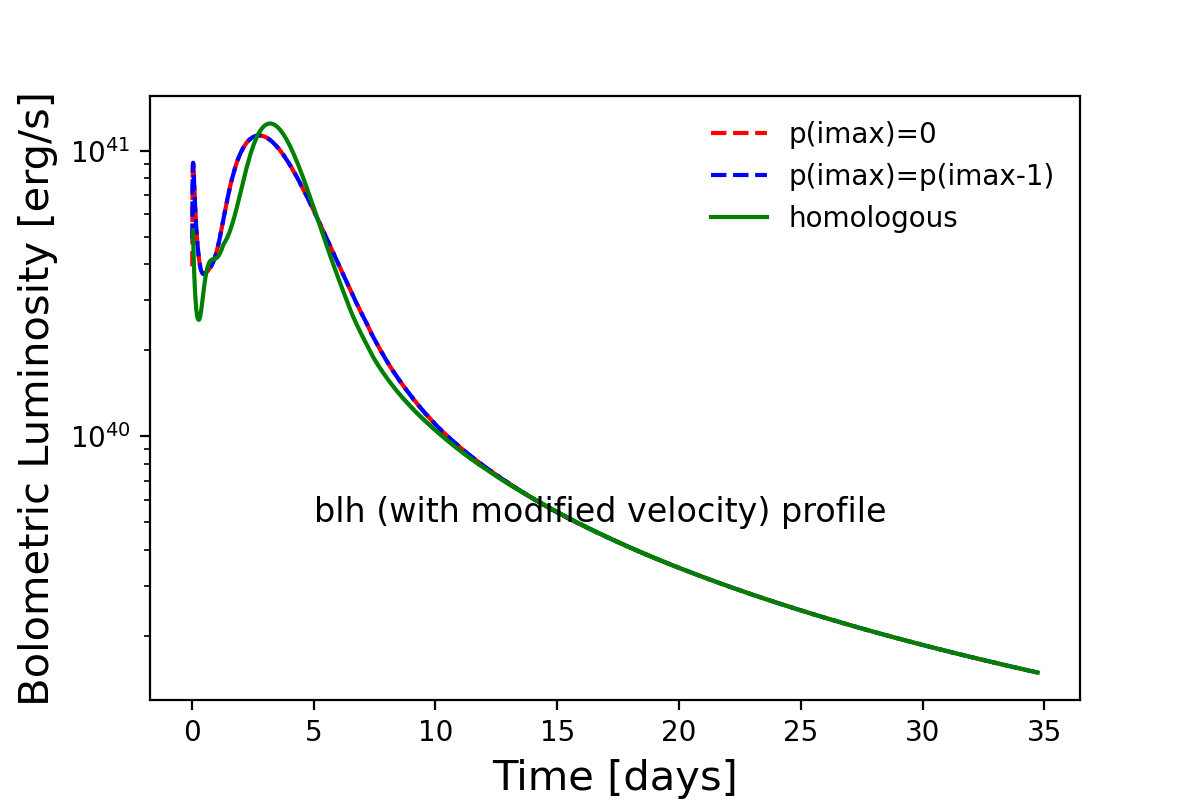
\includegraphics[scale=0.5]{figures/CodeValidation-Hydrodynamics/LC_blh-mvel_cb_zb_homologous.png}
\caption{Homologous Expansion VS Hydrodynamic Evolution: blh (with modified velocity)}
\label{CodeValidation-Hydro_blh-mvel}
\end{figure} 


\begin{figure}
\centering
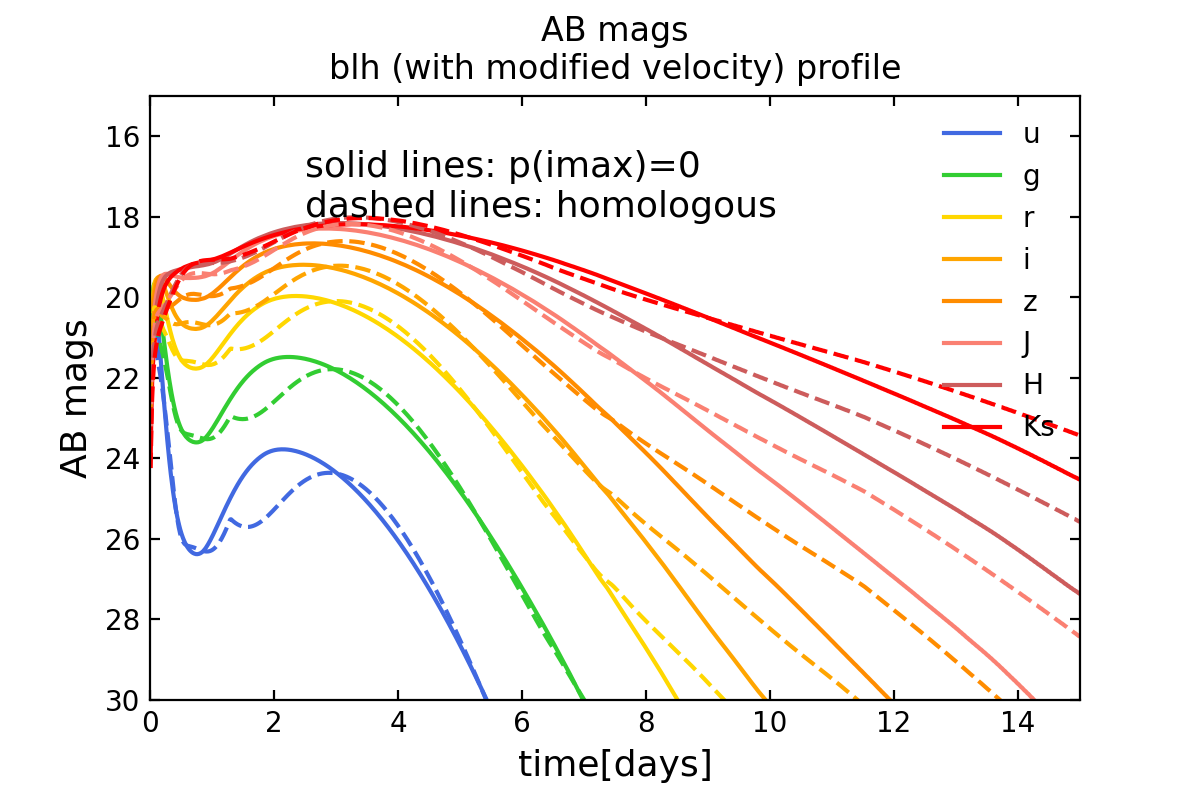
\includegraphics[scale=0.5]{figures/CodeValidation-Hydrodynamics/ABmags_blh-mvel_zb_homologous.png}
\caption{Homologous Expansion VS Hydrodynamic Evolution, multicolor: blh (with modified velocity) }
\label{CodeValidation-Hydro_ABmags_blh-mvel}
\end{figure} 


see Figure \ref{CodeValidation-Hydro_wind3ex3-Tex3}, Figure \ref{CodeValidation-Hydro_blh-mvel}, Figure \ref{CodeValidation-Hydro_ABmags_blh-mvel}

\subsection{Energy conservation}

The energy conservation equation in hydrodynamics is 

 \begin{equation}
 \label{conservation_1}
 \begin{aligned}
 	 	\frac{\mathrm{d}}{\mathrm{d} t} \int_{\Omega} \rho\left(\epsilon+\frac{1}{2} \boldsymbol{v}^{2}\right) \mathrm{d} V & =\int_{\Omega} \rho \boldsymbol{f_b} \cdot \boldsymbol{v} \mathrm{~d} V -\int_{\partial \Omega} p \boldsymbol{v} \cdot \mathrm{d} \boldsymbol{S} \\&-\int_{\partial \Omega} \boldsymbol{f_s} \cdot \mathrm{d} \boldsymbol{S}+\int_{\Omega} \rho q \mathrm{~d}V
 \end{aligned}
 \end{equation}
 
 Here the surface force $\boldsymbol{f_s}$ = 0 and the body force $\boldsymbol{f_b}$ is the gravitational force. $\epsilon$ represents specific internal energy and $q$ is the heating term including r-process heating and radiation. Therefore, we can write energy conservation as
 



\begin{equation}
\label{conservation_2}
	\frac{d}{dt}(E_{int} + E_{kin}+E_{grav}) = \dot Q - \int p \boldsymbol{v} \cdot d \boldsymbol{S} 
\end{equation}
$\dot Q = H - L_{bol}$, $H$ is the heating from decay of r-process elements and $L_{bol}$ is the bolometric luminosity. For $p_{imax}=0$ boundary condition, the pdV term $-\int p \boldsymbol{v} \cdot d \boldsymbol{S} = p_{1} dV = p_{1} v_1 4\pi r_1^2$  
Integrate Equation (\ref{conservation_2}) over time, we have cumulative energy conservation shown in Figure \ref{energy_conservation}.
 

\begin{figure}
\centering
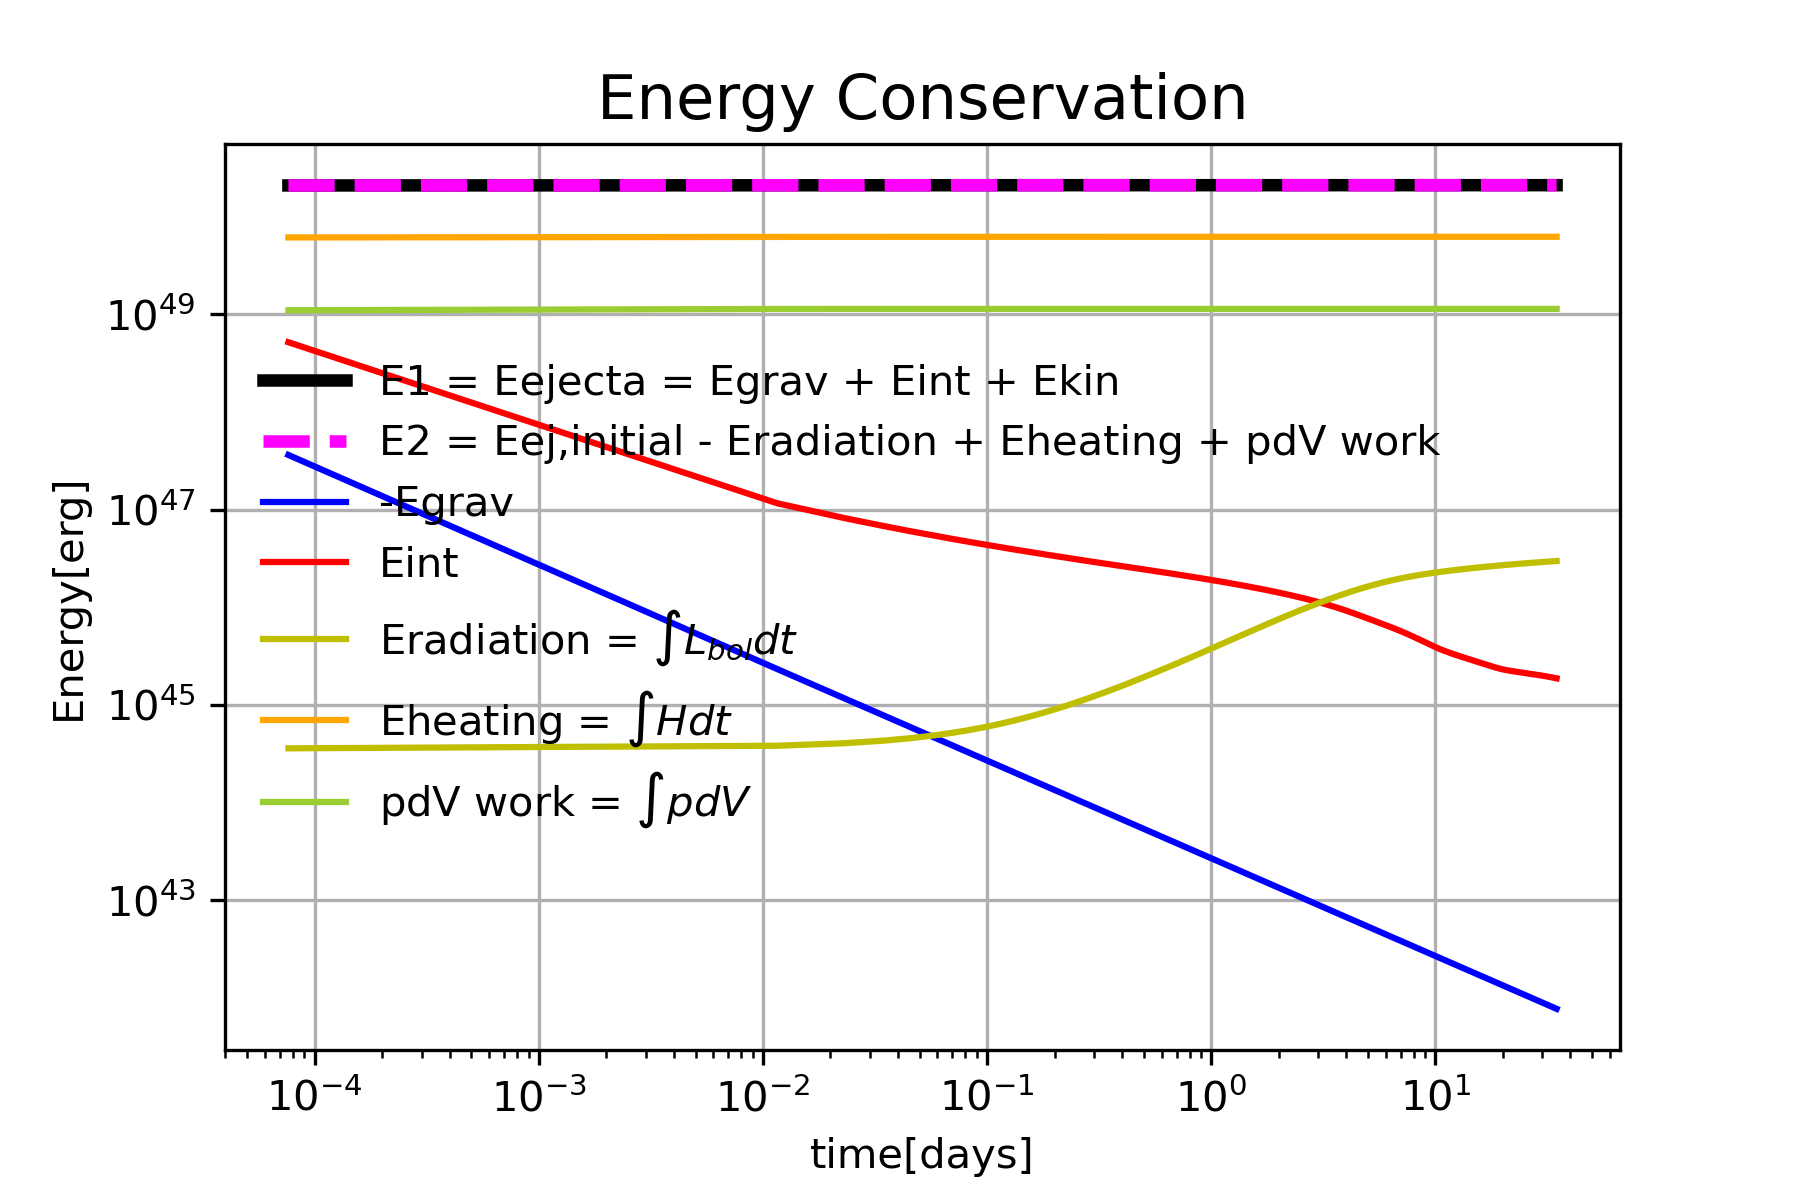
\includegraphics[scale=0.6]{figures/energy_conservation_wind3_Apr2.png}
\caption{Energy conservation of wind3 ejecta ($0.01M_{\odot}, v_{max}=0.2c, Y_e=0.05, s=10\ \mathrm{k_B}, \tau=10\ \mathrm{ ms}$), using $p_{imax}=0$ boundary condition. $E_1$ is the total energy of the ejecta, $E_2$ is the initial ejecta energy + energy from heating - luminosity + pdV work at inner boundary. The maximum difference between $E_1$ and $E_2$ is 0.015\%.}
\label{energy_conservation}
\end{figure}



\subsection{Comparison with analytic models}
\begin{itemize}
    \item ZW: to determine an "optimal" wind profile to be handed over to GR and RK
    \item GR, RK: to run the analytical models
\end{itemize}

\begin{figure}
    \centering
    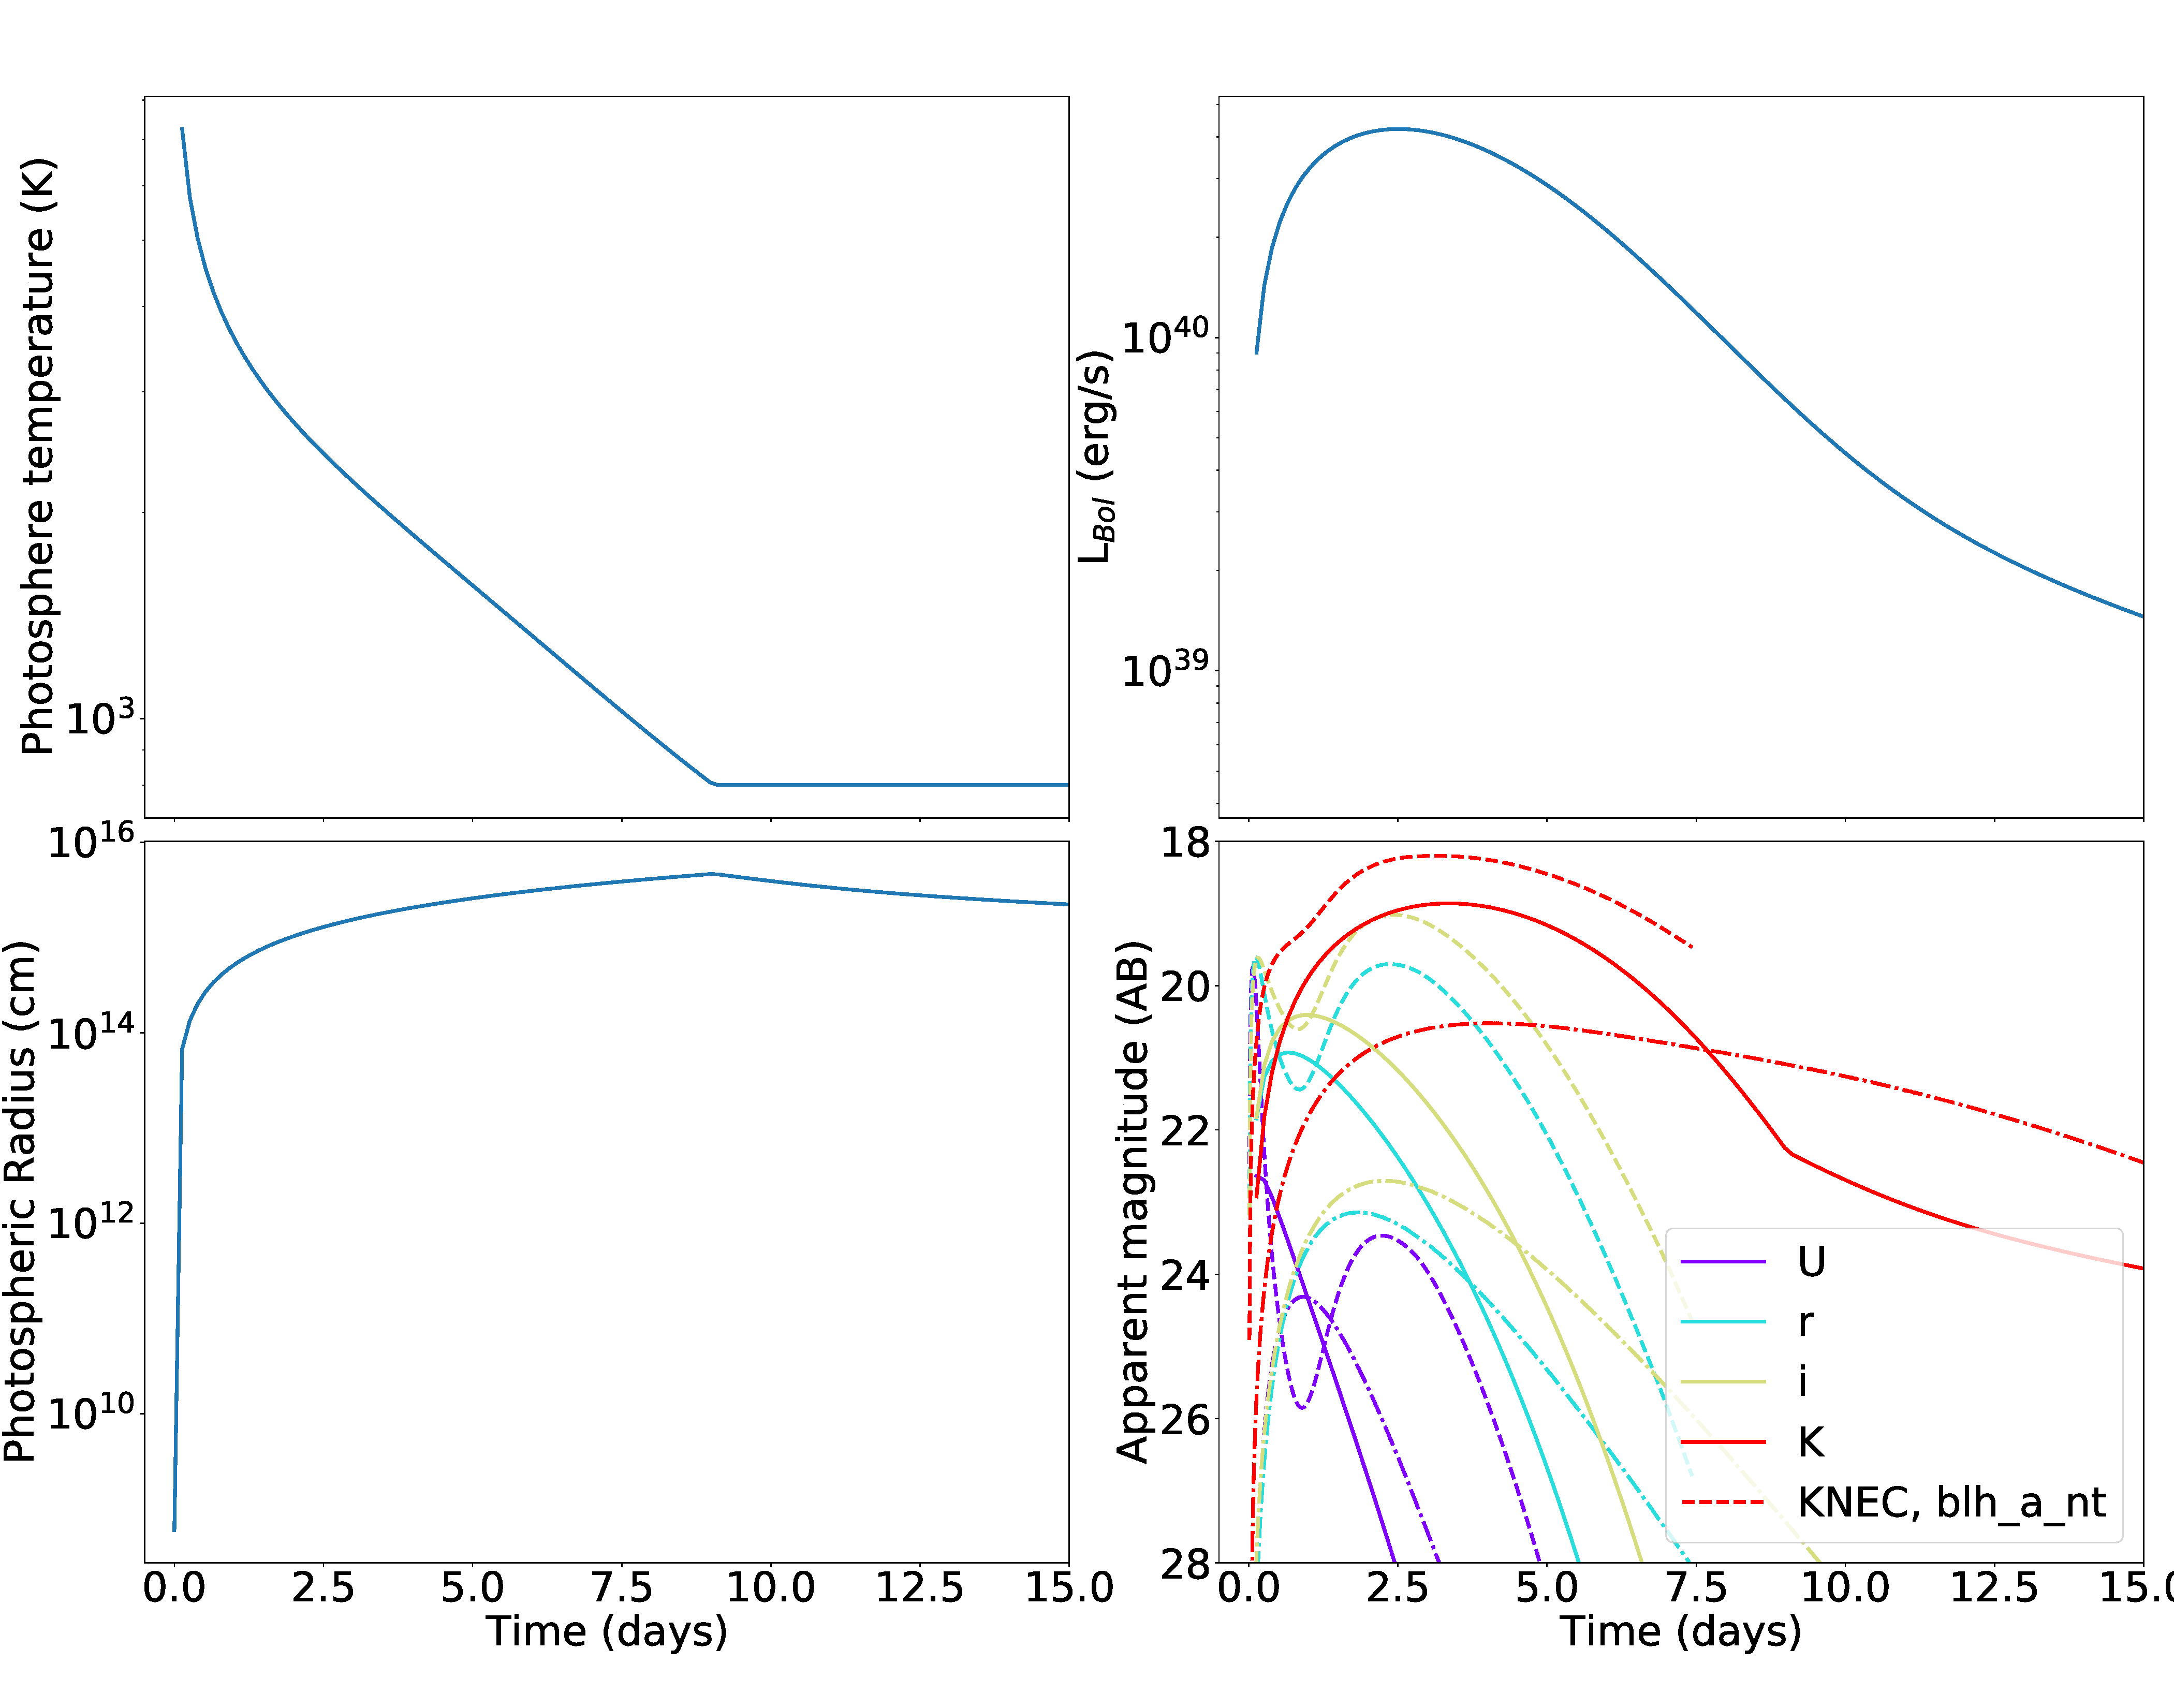
\includegraphics[width=0.45\textwidth]{figures/LC_1comp_wind3_mej-0.01_vej-0.2_kappa_10_KNEC_blh_a_nt.pdf}
    \caption{Caption}
    \label{fig:analytical_comparison}
\end{figure}


% ===========================================================================
\section{Ab-initio simulations: from mergers to kilonovae}
% ===========================================================================
\subsection{General features}
\subsection{Impact of uncertainties in the heating rates}
\begin{itemize}
    \item ZW: to redo the analysis of the heating rate by tweaking the latest heating rates and using the wind profile
    \item ZW: consider a couple of cases ("low" and "high" Ye)
    \item ZW: compare hydro profiles when heating rates are the same
    \item ZW: bonus: consider testing the case with no hydro evolution
\end{itemize}

% ===========================================================================
\section{A first application to AT2017gfo}
% ===========================================================================
\subsection{Best fitting analytical models}
Not sure we want this

\subsection{Comparison between NR informed models and observations}
\begin{itemize}
    \item ZW: compare vanilla and time extended models to observations
    \item DR: to provide a DD2 profile from the spiral-wind paper
    \item ZW: consider how changes in opacities and/or heating rates could affect the comparison
\end{itemize}

\subsection{Impact of shock cooling}
\begin{itemize}
    \item ZW: look at parameters used in Beloborodov+ and Piro+
    \item ZW: try with BLh profile
\end{itemize}

% ===========================================================================
\section{Conclusions}
% ===========================================================================

\bibliographystyle{mnras}
\bibliography{references}


% Don't change these lines
\bsp	% typesetting comment
\label{lastpage}
\end{document}

% End of mnras_template.tex
